% Условная компиляция для самостоятельной работы
\ifdefined\mainfile
    % Если это часть основного файла, не добавляем начало и конец документа
\else
    \documentclass[12pt, a4paper]{report}
    \usepackage{/Users/vladbelousov/Desktop/Semestr_4-FP-NSU/Настройка/library}
    \usepackage[utf8]{inputenc} % Подключение поддержки UTF-8
    \begin{document}
\fi

%%-------------------------------%%

\[ \vec{E } (\vec{r } ,t ) = \vec{E } (x, y ) e^{ i k_z z - i \omega y }, \text{ } \vec{B } (\vec{r } , t )= \vec{B } (x,y) e^{  i k_z z - i \omega t}    \] 

\[ \nabla_{ \perp  } (E_z (x,y ) e^{ i k_z z })   - \frac{\partial}{\partial  z } (\vec{E } _{ \perp } (x,y ) e^{ i k_z z }) =  \frac{ i \omega}{c }[ \vec{e_z} \times  \vec{B} _{ \perp } (x,y ) e^{ i k_z z}  ]   \] 

\[ 1)\quad  \nabla_{ \perp } E_z (x, y ) - i k_z \vec{E } _{\perp  } (x,y   ) = \frac{ i \omega }{c } [ \vec{e_z} \times  \vec{B} _{ \perp } (x,y ) ]   \] 

\( \displaystyle \mathrm{rot } \vec{H } = \frac{i \omega \varepsilon (\omega)}{c } \vec{E}  \to  \)  домножим на \( \displaystyle \mu (\omega)  \Rightarrow \mathrm{rot } \vec{B } = - \frac{i \omega }{c } \varepsilon (\omega ) \mu (\omega) \vec{E }   \), далее аналогично домножаем векторно на \( \vec{e_z}  \)  и выделяем \( \perp  \) составляющую: 

\[ 2) \quad \nabla_{ \perp } B_z (x,y ) - i k_z \vec{B } _{\perp } (x,y ) = - \frac{i \omega }{c } \varepsilon \mu [\vec{e_z} \times  \vec{E} _{ \perp } (x,y ) ]   \] 

\[ \nabla_{ \perp } E_z (x,y ) - i k_z \vec{E }_{\perp  }(x,y ) = \frac{i \omega }{c } \left[ \vec{e_z} \times \left( \frac{\nabla_{ \perp } B_z (x,y )  + \frac{i \omega \varepsilon \mu}{c } [\vec{e_z} \times  \vec{E} _{ \perp }]  }  {i k_z}  \right) \right] ;     \] 

\[ [\vec{e_z }\times [\vec{e_z }\times  \vec{E } _{\perp  }  ]  ] = \vec{e_z } \cancelto{0}{(\vec{e_z }, \vec{E }_{\perp  }   )} - \vec{E } _{ \perp }  \] 

\[ i k_z \nabla_{ \perp  } E_z (x,y ) + k_z ^2 + \vec{E } _{\perp  } (x,y ) = \frac{ i \omega }{c } [ \vec{e_z } \times \nabla_{ \perp  } B_z (x,y )  ] + \frac{ \omega ^2 \varepsilon \mu }{c ^2 }  \vec{E }_{ \perp }     ( x,y ) ; \quad \ae ^2 = \frac{ \varepsilon (\omega )\mu (\omega ) \omega ^2 }{c ^2 }   - k_z ^2   \] 

\[ \vec{E } _{\perp  } (x,y) = \frac{i k_z }{ \ae ^2 } \nabla_{ \perp } E_z (x,y ) - \frac{ i \omega }{c \ae ^2  } [ \vec{e_z  } \times  \nabla_{ \perp } B_z (x,y ) ]     \] 

\[ \vec{B } _{\perp } (x,y )= \frac{i k_z }{ \ae ^2 } \nabla_{ \perp } B_z (x,y ) + \frac{ i \omega \varepsilon \mu }{c \ae ^2  } [ \vec{e_z  } \times  \nabla_{ \perp } E_z (x,y ) ]     \] 

Уравнения на \( E_z (x,y ) \) и \( B_z (x,y ) \)

\[ \begin{aligned}
\begin{cases}
    \displaystyle \mathrm{rot }(\mathrm{rot }\vec{E } ) = \frac{ i \omega }{c } \mathrm{rot } (\mu \vec{H } ) = \frac{ i \omega }{c }\mu \left( - \frac{ i \omega \varepsilon }{c}  \right) \vec{E}  \\
    \displaystyle \mathrm{rot }(\mathrm{rot }\vec{E } ) = \cancelto{0}{\nabla \mathrm{div } \vec{E }} - \Delta \vec{E }  , \quad  \mathrm{div } \vec{D } = 0 = \mathrm{div } - \varepsilon \vec{E } = \varepsilon \mathrm{div } \vec{E }  =0  
\end{cases}
\quad   \Rightarrow
\end{aligned} \] 

\[ \Rightarrow  \Delta \vec{E } (x,y,z ) + \frac{ \omega ^2 \varepsilon \mu }{c  ^2 } \vec{E } (x,y,z ) = 0  \] 

\[ \left( \frac{\partial}{\partial  x ^2 }+ \frac{\partial}{\partial  y ^2 } \frac{\partial}{\partial  z }   \right) E_z (x,y ) e^{ i k_z z } + \frac{ \omega ^2 }{ c ^2 } \varepsilon \mu E_z (x,y ) e^{ i k_z z } = 0  \] 

\[ \Delta_{\perp  } E_z (x,y ) e^{ i k_z z } - k_z ^2 E_z (x,y  ) e^{ i k_z z }  + \frac{\omega ^2 \varepsilon \mu }{c ^2 } E_z (x,y ) e^{ i k_z z } = 0     \] 

\[ \Delta_{\perp  } E_z (x,y )  + \ae ^2 E_z (x,y  )  = 0    - \text{ двумерное волновое уравнение}  \] 

\[ \text{Аналогично: } \nabla_{ \perp  } B_z (x,y ) + \ae ^2 B_z (x,y ) = 0 \] 

Граничные условия: 

\begin{center}
    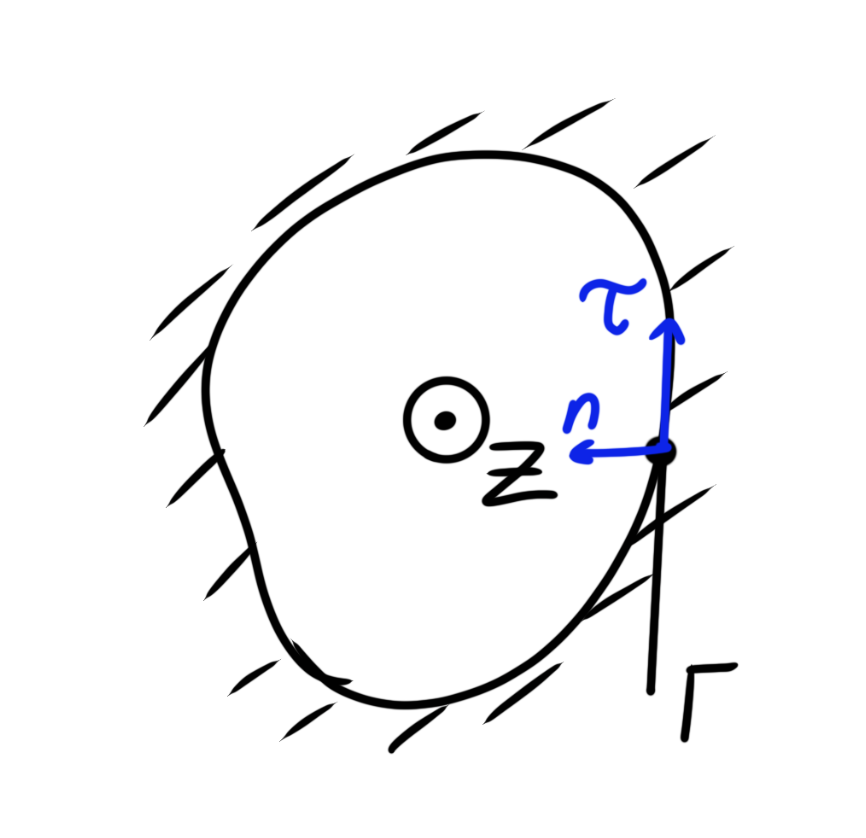
\includegraphics[width=0.3\textwidth]{/Users/vladbelousov/Desktop/Semestr_4-FP-NSU/ЭиО/Лекции_по_дням/image/54.png}
\end{center}


\[ E_{\tau }|_{\text{Г} }  = 0 \Rightarrow (\vec{E } , \vec{r } ) = 0  ,\quad  (\tau -\text{ вдоль поверхности}) , \quad  B_{n } |_{\text{Г} } = 0  \Rightarrow (\vec{n } , \vec{B } )|_{\text{Г} } = 0  \] 

\[ \text{Пусть } \vec{\tau } \parallel \vec{e_z } \Rightarrow E_z (x,y ) e^{i k_z z - i \omega t} |_{\text{Г} } = 0 \Rightarrow E_z (x,y ) |_{\text{Г} } = 0    \] 

\[ \text{Пусть }\vec{\tau} \cancel{\parallel} \vec{e_z } \Rightarrow E_{\tau }  = ( \vec{\tau }, (\vec{e_z }E_z + \vec{E } _{\perp }  ) ) |_{\text{Г} } = \underbrace{(\vec{\tau }, \vec{e_z}  ) \cancelto{0}{E_z}|_{\text{Г} }}_{0}  +(\vec{\tau }, \vec{ E } _{\perp }  )   \] 

\[ = \left( \vec{\tau} , \left\{ \frac{i k_z }{\ae ^2 } \nabla_{ \perp } E_z(x,y ) - \frac{ i \omega }{c \ae ^2 } [ \vec{e_z } \times  \nabla_{ \perp } B_z (x,y )  ]   \right\} \right)  \bigg | _{\text{Г} }  = \frac{ i k_z }{\ae ^2 } \frac{\partial  E_z}{\partial \tau }\bigg | _{\text{Г} } - \frac{ i \omega  }{c \ae ^2 } ( \vec{\tau }, [ \vec{e_z } \times  \nabla_{ \perp } B_z (x,y )] ) \bigg | _{\text{Г} } =\] 

\[ \pm  \frac{ i \omega }{c \ae ^2 }( \nabla B_z , \vec{n } ) \bigg | _{\text{Г} }  = \pm  \frac{ i \omega  }{c \ae ^2 } \frac{\partial  B_z(x,y )}{\partial  n } \bigg | _{\text{Г} } = 0 \Rightarrow E_z (x,y )\bigg | _{\text{Г} } = 0, \frac{\partial  B_z}{\partial  n }  \bigg | _{\text{Г} } = 0   \] 

Второе граничное условие: 

\[ (\vec{n } , \vec{B } ) \bigg | _{\text{Г} } = 0 \Rightarrow \left( \vec{n } , \left\{ \vec{e_z }B_z (x,y ) + \frac{ i k_z }{\ae ^2 } \nabla_{ \perp } B_z (x,y ) + \frac{ i \omega \varepsilon \mu }{c  \ae ^2 } [ \vec{e_z }\times  \nabla_{ \perp } E_z (x,y ) ]    \right\} \right) \bigg | _{\text{Г} } =\] 

\[ \frac{i k_z }{\ae ^2 } \frac{\partial  B_z (x,y )}{\partial  n} \bigg | _{\text{Г} } + \frac{ i \omega \varepsilon \mu}{ c \ae ^2 } ( \vec{n }, [ \vec{e_z } \times  \nabla_{ \perp } E_z (x,y )] ) \bigg | _{\text{Г} }   = \frac{ i \omega \varepsilon \mu  }{c \ae ^2 } \frac{\partial  E_z (x,y )}{\partial  n } \bigg | _{\text{Г} } = 0  \] 

Для упрощения анализа разделим общее решение на два: 

1-ый тип: \( E  \) - волна (ТМ - волна) \( E_z (x,y  ) \neq 0 , B_z (x,y  ) = 0  \)  внутри волновода;

2-ой тип: \( H  \) - волна (ТЕ - волна) \( E_z (x,y  ) = 0 , B_z (x,y  ) \neq 0  \)\dots

Для \( E  \) - волны: \(\Delta_{ \perp  } E_z (x,y  ) + \ae ^2 E_z (x,y ) = 0 + \text{ Г.У } E_z |_{\text{Г} }   = 0 \) 

- задача Штурмана-Лиувилля, из решения которой находятся собственные значения \( \ae_{n } , n= .... \) и собственные функции \( E_{z } ^{(n )}  (x,y) \) 

Для \( H  \) - волны: \(\displaystyle  \Delta _{\perp } B_z (x,y) + \ae ^2 B_z (x,y ) = 0 + \text{ Г.У. } \frac{\partial  B_{z } }{\partial  n } |_{\text{Г} } =0   \) 

Пример 1: \( H  \) - волна в прямоугольном волноводе

\begin{center}
    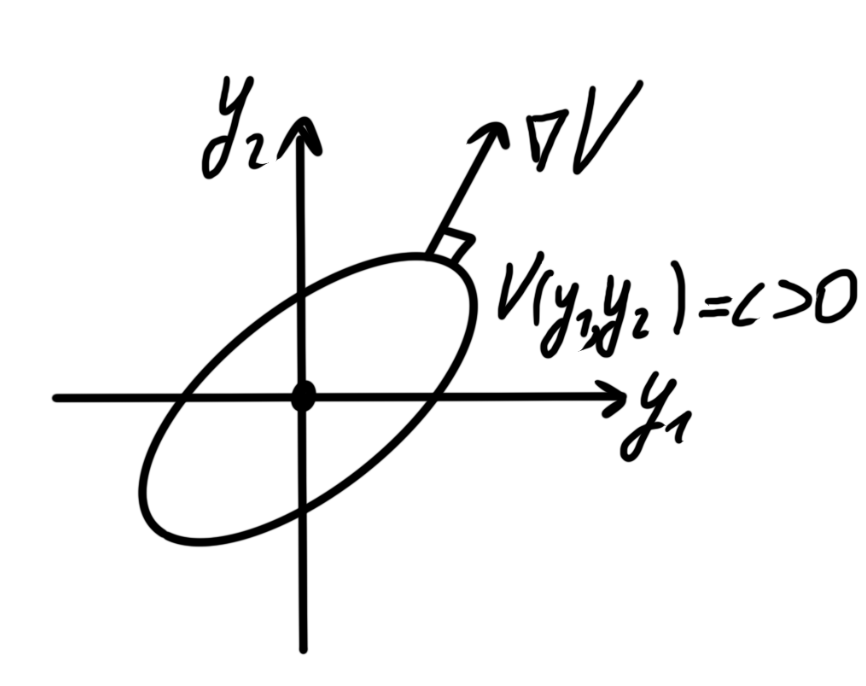
\includegraphics[width=0.4\textwidth]{/Users/vladbelousov/Desktop/Semestr_4-FP-NSU/ЭиО/Лекции_по_дням/image/55.png}
\end{center}

\[ \left(  \frac{\partial  ^2 }{\partial  x ^2 } + \frac{\partial  ^2 }{\partial  y  ^2 }   \right) B_z (x,y ) + \ae ^2 B_z (x,y) = 0 , \text{  } + \text{ Г.У. } \frac{\partial  B_{z } }{\partial  n } |_{\text{Г} } =0  \Rightarrow \frac{\partial  B_z }{\partial  x }|_{x=0,a} = 0, \text{ } \frac{\partial  B_z }{\partial  y }|_{y=0,b} = 0     \] 

Пусть \( B_z (x,y  )= B_1(x)B_2(y) \) 

\[ B_2(y )B_1 '' (x) + B_1( x) B_2 '' (y )+ \ae ^2 B_1(x) B_2(y ) = 0 \] 

\[ \Rightarrow \underbrace{\frac{ B_1 '' (x )}{B_1 (x)} }_{=\mathrm{const} = -k_x ^2   }+\underbrace{\frac{ B_2 '' (y )}{B(y )}}_{=\mathrm{const}= - k_y ^2  } + \ae ^2 = 0   \Rightarrow \begin{cases}
    B_z (x,y ) = B_0 \sim (k_xx \alpha_x  ) \sin ( k_y y \alpha_y ) \\ 
    \ae ^2 = k_x ^2 + k_y ^2 
\end{cases} \] 

Граничные условия: 

\[ \frac{\partial  B_z }{ \partial  x } \bigg | _{x = 0  } = k_x B_0 \cos \alpha_x \sin  (k_y y + \alpha_y ) = 0 \text{ при } \forall  y \Rightarrow \alpha_x = \frac{\pi}{2}     \] 

\[ \frac{\partial  B_z }{\partial  x } \bigg | _{x = a  } = k_x B_0 \cos (k_x a + \frac{\pi}{2 } )\sin( k_y y + \alpha_y ) = 0 \Rightarrow k_x a = n_x \pi, \text{ }  k_x =  \frac{ n_x \pi } {a } , \text{ }  n_x \in  \mathbb{Z} \] 

\[ \text{Аналогично: }  \alpha_y = \frac{\pi}{2 } , \text{ } k_y = \frac{ n_y \pi } {b } , \text{ }  n_y \in  \mathbb{Z} \Rightarrow \ae_{n_x, n_y } = \sqrt{\left( \frac{n_x \pi }{a }  \right) ^2 + \left( \frac{n_y \pi }{b } \right) ^2} - \text{собственные числа} \] 

\[ B_z (x,y  ) = B_0 \cos (k_x x ) \cos (k_y y ) , \text{ }  B_z(\vec{r }  ,t )= B_0 \cos (k_x x ) \cos (k_y y) e^{i k_z z - i \omega t} \] 

\[ E_{\perp } (x,y  ) = - \frac{i \omega          }{c \ae _{n_x, n_y } ^2 }[\vec{e_z  } ^2 \times  \nabla_{ \perp } B_z (x,y ) ] , \text{ } B_{ \perp  } (x,y )= \frac{ i k_z }{\ae ^2 } \nabla_{ \perp } B_z(x,y)    \] 

\[ \nabla_{ \perp } B_z(x,y) = \left( \vec{e_x } \frac{\partial  }{\partial  x } + \vec{e_y } \frac{\partial  }{\partial  y }   \right) B_z(x,y )=- B_0 \left\{ \vec{e_x }k_x \sin (k_x x ) \cos (k_y y ) + \vec{e_y }k_y \cos (k_x x ) \sin (k_y y )  \right\} \] 

Какие \( n_x, n_y  \) допустимы?  Пусть \( n_x = 0 , n_y = 0 \) 

\[B_z(\vec{r },t ) = B_0 e^{i k_z z - i \omega t }, \text{ } \vec{B } _{\perp  }(\vec{r } ,t ) = \frac{ i k_z }{0 ^2 } 0 - \text{ проверить из уравнений Максвелла, что  } B_{\perp  } = 0       \] 

\[ \mathrm{div} \vec{B } = 0 = \frac{\partial  B_z }{\partial  z } = i k_z B_0 e^{i k_z z - i \omega t } (k_z \neq 0 ) \Rightarrow B_0 \text{ } (\text{такой моды нет} )   \] 

Пусть: \( \displaystyle  n_x = 1 , n_y = 0  \Rightarrow \ae _{1,0 } = \frac{\pi}{a}, \text{   }  \frac{ \omega_{1,0 } ^2 \varepsilon \mu }{c ^2 } = \left(  \frac{\pi }{a }  \right) ^2 + k_z ^2  \) 

\[ B_z ( x,y ) = B_0 \cos (k_x x ) ,\text{ } B_{\perp  } (x,y) = \frac{i k_z }{\ae_{1,0} ^2 } B_0 (- k_x  )\sin (k_x x )\vec{e_x} , \text{  далее } \to  \begin{cases}
\varepsilon(\omega ) = \mathrm{const }  \\
\mu (\omega ) = \mathrm{const } 
\end{cases}    \] 

\[ \vec{E } _{ \perp  }(x,y ) = - \frac{ i\omega }{c \ae ^2 } \vec{e_y }B_0 (-k_x )\sin (k_xx)    \] 

\begin{center}
    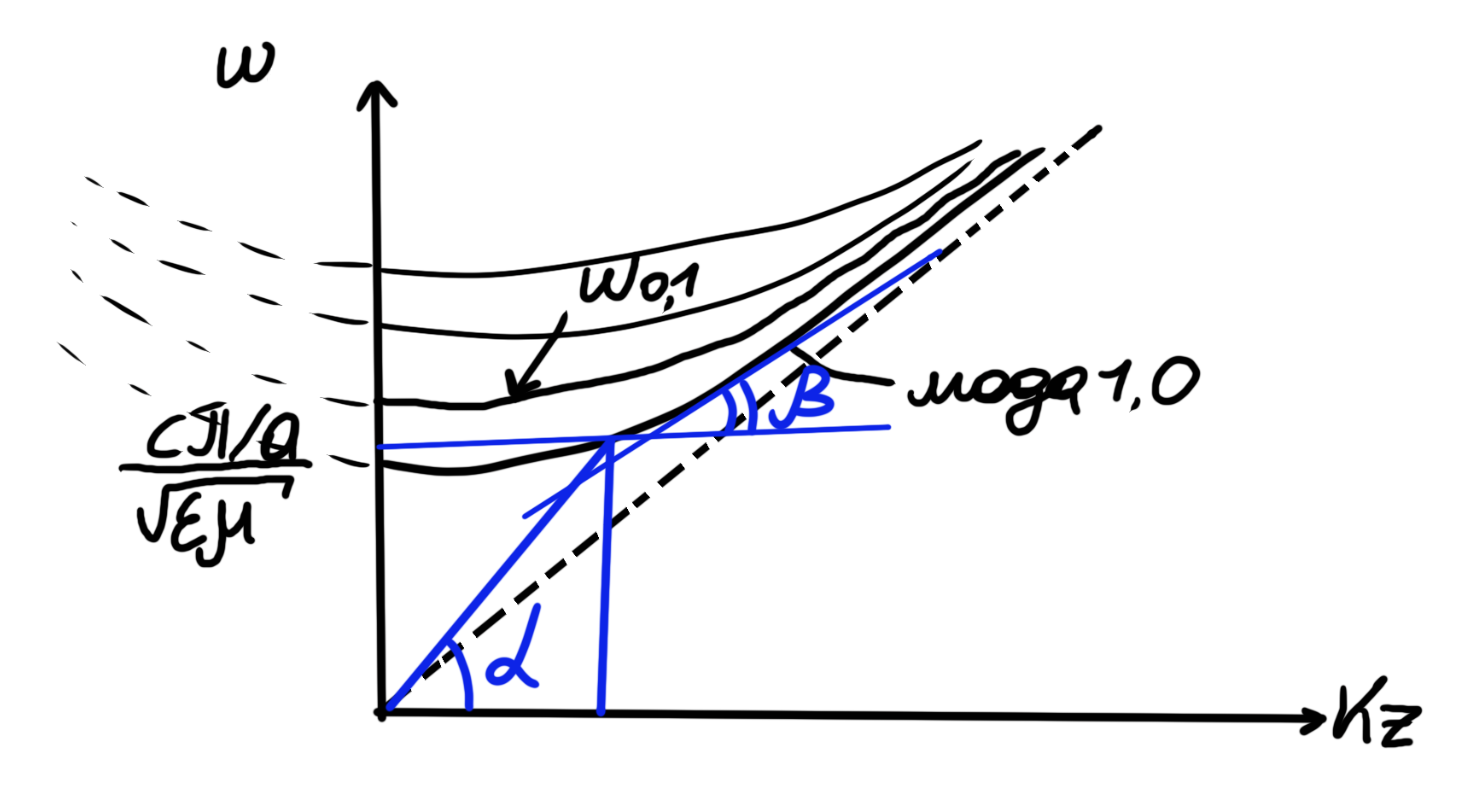
\includegraphics[width=0.5\textwidth]{/Users/vladbelousov/Desktop/Semestr_4-FP-NSU/ЭиО/Лекции_по_дням/image/56.png}
\end{center}

- мода\( _{1,0}  \) - основная мода волновода.

\[ v_{\Phi } = \frac{ \omega } {k_z }, \text{  } v_{g } = \frac{ d \omega }{d k_z}   \]

\[ v_{\Phi } v_g = \frac{ c_2 }{\varepsilon \mu}   \] 

\[ v_{\Phi } = tg \alpha , \text{ }  v_g =  tg \beta \] 

Представление в виде плоских волн: 

\[ B_z (\vec{r }, t ) = B_0 \left( \frac{ e^{i k_x x } + e^{-i k_x x } }{2} \right) e^{i k_z z - i \omega t}  = \frac{B_0 }{2 } e^{ i k_xx + i k_z z - i \omega t} +  \frac{B_0 }{2 } e^{-i k_xx - i k_z z - i \omega t}\]

\begin{center}
    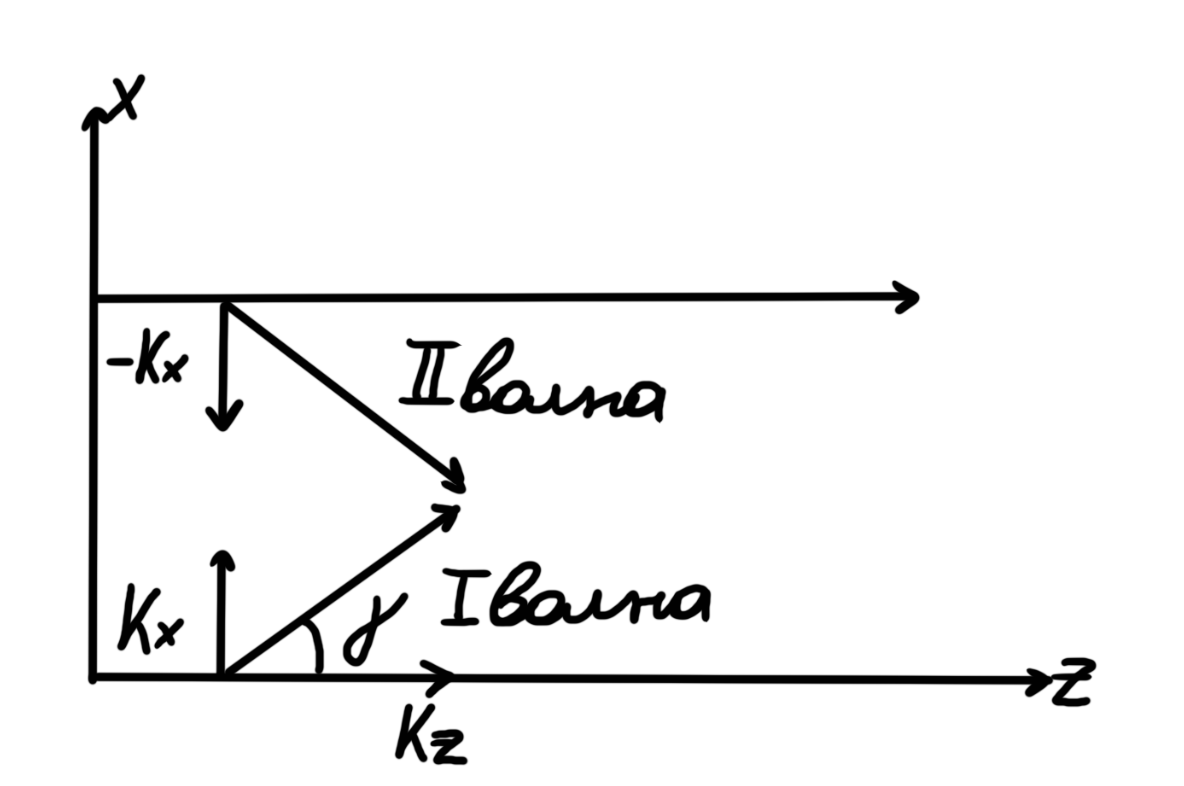
\includegraphics[width=0.5\textwidth]{/Users/vladbelousov/Desktop/Semestr_4-FP-NSU/ЭиО/Лекции_по_дням/image/57.png}
\end{center}

\[ v_{\Phi } = \frac{c }{ \sqrt{\varepsilon \mu   }\cos \gamma}  , \quad  v_g = \frac{c }{ \sqrt{\varepsilon \mu  }}\cos \gamma , \cos \gamma = \frac{ k_x }{\sqrt{k_x ^2 + k_z ^2 }}   \] 

%%-------------------------------%%

% Закрытие документа, если файл компилируется отдельно
\ifdefined\mainfile
    % Если это основной файл, не нужно заканчивать документ
\else
    \end{document}
\fi